\documentclass[12pt, letterpaper]{article}
\usepackage{bbold}
\usepackage{indentfirst}
\usepackage{amsmath, amssymb}
\usepackage[T1]{fontenc}
\usepackage[utf8]{inputenc}
\usepackage{physics}
\usepackage{tensor}
\usepackage{braket}
\usepackage{graphics}
\usepackage{grffile}
\usepackage[export]{adjustbox}
\usepackage{svg}
\usepackage{caption}
\usepackage{subcaption}
\usepackage{authblk} 
\usepackage{blindtext}
\usepackage{setspace}
\title{\color{blue}A Research Project on \\ "Bose-Einstein Statistics"}

\author{ COURSE CODE : TP-407 \\ \textbf{SUBMITTED BY}
 \\  CLASS ROLL : SH-098-015 \  EXAM ROLL: 30210 \\
 REGISTRATION NUMBER : 2016-814-701 \\     SESSION : 2016-17
\\ 
\includegraphics[width=0.3\textheight]{DU.jpg} \\  DEPARTMENT OF THEORETICAL PHYSICS \\ UNIVERSITY OF DHAKA 
}
\doublespacing

\begin{document}
    \maketitle
    \section*{Contents}
    \subsection*{(i) Abstract}
    \subsection*{(ii) Section-1 : Introduction and Historical Background}
    \subsection*{(iii) Section-2 : Bose-Einsteien Distribution function and Plank's law of radiation for black-body on the basis of Bose's papaer}
    \subsection*{(iv) Section-3 : Some statistical calculation based on Bose-Eistein distribution}
    \subsection*{(v) Section-4 : Bose-Einstein Condensate}
    \subsection*{(vi) Section-5 : Einstein's papers on the basis of Bose-Einstein statistics}
    \subsection*{(vii) Summary}
    \subsection*{(viii) Reference}
    \newpage
    \section*{Abstract}
        In June 1924, Einstein received a letter from a Bengali physicist,
        Satyendra Nath Bose, who asked him politely to translate—if he believed it
        was worth it—and forward for publication a paper on the hypothesis of light
        quanta, which he had attached. Einstein complied and translated and sent
        to Zeitschrift für Physik on behalf of Bose. Einstein then extended Bose's ideas to ideal gas in two other papers.
        He published totally three papers on this. Einstein developed the analogy between gas and radiation.
        We will discuss Bose's and Einstein's those papers which contains Planks law of radiation, Bose Einstein
        distribution, Bose-Eistein Condensate, Quantum theory of mono-atomic ideal gas etc. 
        \newpage
    \section*{Section - 1}
    \subsection*{Introduction and Historical Background}
    \noindent
    ------------------------------------------------------------------------------ \\ 
    \\
    \\
    \\


    \subsection*{Introduction}
    
    Bose-Einstein statistics is a procedure for counting the possible states of quantum systems composed of identical particles with integrer
    spin and Bose-Einstein distribution is the one of the two possible ways in which a collection of indistinguishable particles may occupy a set 
    of availabe discrete energy states.\\

    It takes it name from S.N. Bose, the Indian Physicist, who first proposed it for light quanta(1924), and Albert Einstein, who extended
    it to gas molecules. Both in classical and in quantum mechanics, the behavior of systems composed of a large number of particles 
    can be investigated with the help of statistical consideratoins.If all particles obey the same dynamics and if there interactions 
    can be neglected, in a first apporximation,one can determine all possible energy states of a single particle and then make statistical
    assumptions on the distribution of particles among single particle states, thus computing the average behavior of the whole system.\\
    
    The usual statistical assumptions is that, all possilbe states of many particle system (all configuration) are equally probable.
    As became clear around the middle 1920's, the description of quantum systems of many particle has to be different from that of the classical
    ones, a fact usually describe by refereing to the "indistinguishability" of quantum particles to the "distingushability" of classcial particles.\\

    
    
    \subsection*{Historical Background}

    In 1921, S.N. Bose, joined as a Reader(Professor without a chair) of the deptartment of physics of \ the recently founded University Of Dhaka.\
    He along with astrophysicist Meghnad Saha, presented several papaers in theoretical physics and pure mathematics from 1918, onwards.\\

    In 1924, while working as a reader, Bose  wrote a paper deriving Plank's quantum radiation law without any reference of classical 
    physics, by using a novel way of counting the states of identical particles. \\ 
    This paper was seminal in creating the important field of quantum statistics. Though not accepted once
    for publication, he sent the article directly to A. Einstein in Germany. \\

    Einstein recognising the importance of the paper, translated it into German by himself, and submitted it on Bose's behalf to the 
    prestigious "Zeitschrift fur Physik". As a result, of his recognition Bose was able to work for two years in Europian X-Ray and 
    Crytalography laboratories, during which he worked with Louis De Broglie, Mary Courie, and Eistein.\\
    
    The idea was developed by Bose in such way that, while presenting a lecture at the University of Dhaka on the Plank's radiation law
    and the Ultraviolte catastrophe, Bose inteded to show his students that the contemporary theory was inadequate, beacause it predicted
    results not in accordance with experimental results. In the process of describing this discrepency, Bose for the first time took 
    the position that, The Maxwell-Boltzman disthvribution would not be true for microscopic particles, where fluctuation due to 
    Heisenberg's uncertainity principle will be significant. Thus he stressed the probability of finding particles in the phase space,
    each states having volume $h^{3}$, and descarding the distinct position and momonetum of the particles. \\
    
    The reason Bose's interpretaion produced accurate results was that, since photons are indistiguishable. This result derived by Bose 
    laid the foundation of quantum statistics. \\ 

    When Einstein met Bose face to face, he asked him whether he had been aware that he had invented a new type of statistics and
    he very candidly said "No". Einstein also did not at first realise how radical the deperture was. But after  Einstein's second paper
    using Bose's method in which Einstein predicted the Bose-Einstein condensation, he started to realise how radical it was and he
    compared it to the wave-particle duality saying that, "Some particles do not behave exactly like partilces." \\ 

    Eistein adopted this idea and extended it to the atoms. This led the prediction of the exsistence of the phenomena which become known
    as Bose-Einstein condensate, a dense collection of bosons which was demonostrated to exist by experiment in 1995. \\ 

    \newpage

    \section*{Section -2 :}
    \subsection*{Bose-Einsteien Distribution function and Plank's law of radiation for black-body on the basis of Bose's papaer.}
    \noindent
    --------------------------------------------------------------------------------------------------- \\ 
    \\
    \\
    \\

    \subsection*{Bose-Einstein Distribution}
    Let us consider an assembly of N bosons and those are distributed as $n_{1}, \  n_{2} ....., \  n_{i} $ into the energy level
    $\epsilon_{1}, \  \epsilon_{2}, ........., \ \epsilon_{i}, $ which has degenerecies $g_{1}, \ g_{2},
    ......, \  g_{i}$. \\ 
    
    So. we can write, 

    \begin{equation}
        N = \sum _{i} n_{i}
    \end{equation}
     
    and,

    \begin{equation}
        E =  \sum _{i} n_{i} \epsilon _{i  }
    \end{equation}

    where, N and E denotes total number particles and total energy respestively.\\

    Now, probability of occupancy of a state at energy level $\epsilon _{i}$ , is simply 
    
    \begin{equation}
        f_{i} = \frac{n_{i}}{g_{i}}
    \end{equation}

    which is actually is the distributuin function.\\

    Since Pauli's exclusion principle is not apllicable to the bosons, so any  number of particles can go
    into a single energy state. \\
    
    If we have 'g' number of states in a energy level then there will be (g-1) number of partitions.\\
    
    Hence, the number of distinct permutations of {n+(g-1)} objects in which we have 'n' identitical items of one type
    and (g-1) identitcal items of another type, will be 

    \begin{equation}
        \Omega(n) =  \frac{[n+(g-1)]!}{n!(g-1)!}
    \end{equation}

    Now, for the entire system the total number of ways in which we can accomplish a particular microstate 
    is , 
    
    \begin{equation}
        W(N) =\prod ^{n} _{i=1}  \frac{[n+(g-1)]!}{n!(g-1)!}
    \end{equation}
    
    Now , we have to find those conditoin which maximize this W(N). \\ 
    
    Taking natural logarithm on both side of the eqn. 5

    \begin{equation}
       ln \ [W(N)] =\sum_{i}  [ln \ [n+(g-1)]! - ln \ n! - ln \ (g-1)!]
    \end{equation}

    We can write, 
    (n+g-1) $\simeq$ (n+g)
    because (n+g) >> 1 \\ 

    Using this result and Stirling's apporximation, we get, 
    \begin{equation}
        ln \ [W(N)] =\sum_{i}  [(n+g) \  ln \ [n+g] - n \ ln \ n  -(g-1) \ ln \ (g-1) -1)]
    \end{equation}

    Now if we maximize this, by differentiating, with respect to 'n', we get,  
    \begin{equation}
        \begin{split}
        \delta  [ln \ [W(N)]] & = 0 \\ 
        \implies \sum _{i} [\delta n \ ln \ (n+g) - \delta n \ ln \ n] &  = 0
        \end{split}
    \end{equation}

    We know,
    \begin{equation}
        \sum_{i} n_{i} = N = constant
    \end{equation}

    \begin{equation}
        \therefore \sum_{i} \delta n_{i} = 0
    \end{equation}


    And, 
    \begin{equation}
        \sum_{i} n_{i} \epsilon _{i}= E = constant
    \end{equation}

    \begin{equation}
        \therefore \sum_{i} \delta n_{i} \epsilon _{i} = 0
    \end{equation}

    Now using Langrange method of undetermined multiplier with equation (8), (10) and (12), we get,
    \begin{equation}
        -ln \ (\frac{n+g}{n}) + \alpha +\beta \epsilon = 0
    \end{equation}

    From this, we can easily get
    \begin{equation}
        \begin{split}
        1 + \frac{g}{n} = e^{\alpha +\beta \epsilon} \\
        \therefore \frac{n}{g} = \frac{1}{e^{\alpha + \beta \epsilon} - 1}    
    \end{split}
    \end{equation}

    This is known as Bose-Einstein Distribution function ($f_{B.E}$).

    \begin{adjustbox}{center,caption={},label={somelabel},nofloat=figure,vspace=\bigskipamount}
        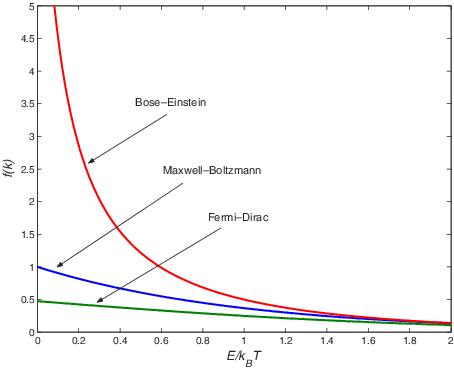
\includegraphics[width=\textwidth]{fig1}
    \end{adjustbox} 

    \newpage

    \begin{adjustbox}{center,caption={},label={somelabel},nofloat=figure,vspace=\bigskipamount}
        \includegraphics[width=0.7\textwidth]{fig2}
    \end{adjustbox}
    
    \begin{adjustbox}{center,caption={},label={somelabel},nofloat=figure,vspace=\bigskipamount}
        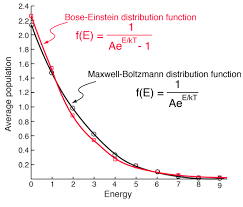
\includegraphics[width=0.7\textwidth]{fig3}
    \end{adjustbox}
     \ \ \ \ \ \ \ \ \ \ \  \ \ \ \ \ \ \  The Bose-Einstein Distribution Graph

    \subsection*{Plank's formula of Black-body radiation using Bose-Einstein distribution}

    In the case of a black body the number of allowed states is 
    \begin{equation}
        g = \frac{4 \pi V p^{2} dp}{h^{3}}
    \end{equation}

    We know, the De Broglie wavelength, 
    \begin{equation}
        \begin{split}
             \lambda &= \frac{h}{p} \\ 
             \therefore dp &= \frac{h \  d\lambda}{\lambda ^{2}}
        \end{split}
    \end{equation}

    putting this value in eqn(15), we get

    \begin{equation}
        g(\lambda) = \frac{4 \pi V d\lambda}{\lambda ^{4}}
    \end{equation}

    This number must be doubled for photon gas because of two states of polarization
    \begin{equation}
        g(\lambda) = \frac{8 \pi V d\lambda}{\lambda ^{4}}
    \end{equation}

    We know, from Bose-Einstein Distribution 
    \begin{equation}
        \frac{n}{g} = \frac{1}{e^{\alpha + \beta \epsilon} - 1}  
    \end{equation}

    and 
    \begin{equation}
        E = nh\upsilon 
    \end{equation}

    combining eqn(18,19,20), we get 
    \begin{equation}
        E(\lambda) = \frac{8 \pi V hc}{\lambda ^{5} (e^{hc/\lambda kT}-1)} 
    \end{equation}

    which is equaivalent to Plank's radiation formula.
    \begin{adjustbox}{center,caption={Plank's law graph},label={somelabel},nofloat=figure,vspace=\bigskipamount}
        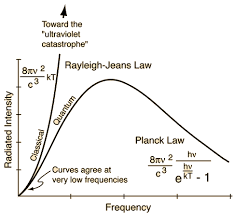
\includegraphics[width=0.7\textwidth]{fig4}
    \end{adjustbox}

    \newpage
    \section*{Section - 3}
    \subsection*{Some statistical calculation based on Bose-Eistein distribution}
    \noindent
    --------------------------------------------------------------------------------------------------- \\ 
    \\
    \\
    \\

    \section*{ Calculation of total number of particles}
    %\section{Model}
    %\section{Discussion}
    %\subsection*{Calculation of total number of particles}
    We know, total number of particles can be written as 
    \begin{equation}
        N = \int f(\epsilon) g(\epsilon) \,d\epsilon 
    \end{equation}

    We know, 
    \begin{equation}
        g(\epsilon) = \frac{d \Omega(\epsilon)}{d\epsilon}
    \end{equation}

    where
    \begin{equation}
        \Omega(\epsilon) = \frac{g_{s}V}{h^{3}} \int 4\pi p^{2} dp
    \end{equation}

    We know,

    \begin{equation}
    \begin{split}
        \epsilon = \frac{p^{2}}{2m}\\ 
        \\
        \therefore  dp = \frac{m d\epsilon}{\sqrt{2m\epsilon} }        
    \end{split}
    \end{equation}

    putting these values, in eqn(23) we get,
    \begin{equation}
        g(\epsilon) = \frac{4\pi m V\sqrt{2m\epsilon}}{h^{3}}
    \end{equation}

    putting the value of $g(\epsilon)$ from eqn(26) and the value of $f_{B.E}$ into the eqn(22), we get, 
    \begin{equation}
        N = \frac{4\pi m V\sqrt{2m}}{h^{3}} \int ^{\infty}_{0} \frac{\sqrt{\epsilon}d\epsilon}{e^{\alpha +  \beta \epsilon}-1}
    \end{equation}

    Now we know, 
    \begin{equation}
        \lambda = \frac{h}{\sqrt{2 \pi m k T}}
    \end{equation}

    usign eqn(28) and letting $\beta \epsilon = x$ we get 
    \begin{align}
        N & = \frac{2V}{\lambda^{3} \sqrt{\pi}} \int \frac{\sqrt{x} dx}{e^{\alpha +x}-1}\\
        \\
            \therefore N  & = \frac{V}{\lambda^{3} } f_{1}(\alpha)
    \end{align}

    where $f_{1}(\alpha)$ is the first order Zeta function.
    
    Zeta function can be written as 
    \begin{equation}
        f_{1}(\alpha) = \sum ^{\infty}_{r=1} \frac{A^{r}}{r^{3/2}} 
    \end{equation}

    We know that $0<A\leq 1$

    $\therefore$  the maximum value of $f_{1}(\alpha)$ is $\approx $ 2.612 at A=1. 

    \begin{align*}
        \therefore N &= \frac{2.612V}{\lambda^{2}} \tag*{(maximum value of A)}\\
        \\
        \therefore N &= \frac{V}{\lambda^{2}} \times A \tag*{(when A << 1)}
    \end{align*}

    \newpage
    \subsection*{Total Energy Calculation}
    We know that 

    \begin{equation}
        \begin{split}
        E =  \sum _{i} n_{i} \epsilon _{i} \\ 
        \therefore E = \int \epsilon f(\epsilon) g(\epsilon) \,d\epsilon 
        \end{split}
    \end{equation}

    We know, from previous section,
    \begin{equation}
        g(\epsilon) = \frac{4\pi m V\sqrt{2m\epsilon}}{h^{3}}
    \end{equation}

    putting the value of $f_{B.E}$  and $g(\epsilon)$ we get
    \begin{equation}
        E = \frac{4\pi m V\sqrt{2m}}{h^{3}} \int ^{\infty}_{0} \frac{\epsilon ^{3/2}d\epsilon}{e^{\alpha +  \beta \epsilon}-1}
    \end{equation}
    Now we know, 
    \begin{equation}
        \lambda = \frac{h}{\sqrt{2 \pi m k T}}
    \end{equation}

    usign eqn(36) and letting $\beta \epsilon = x$ we get 
    \begin{align*}
        E = \frac{4V}{3\lambda^{3} \sqrt{\pi}} \frac{3}{2} kT \int \frac{x^{3/2} dx}{e^{\alpha +x}-1} \\
        \end{align*}
        \begin{align}
        \therefore E = \frac{V}{\lambda^{3}} \frac{3}{2} kT f_{2}(\alpha)
    \end{align}

    where $f_{2}(\alpha)$ is second orer Zeta function.
    Zeta function can be written as
    \begin{equation}
        f_{2}(\alpha) = \sum ^{\infty}_{r=1} \frac{A^{r}}{r^{5/2}} 
    \end{equation}

    Now we have,
    \begin{equation}
        E = \frac{V}{\lambda^{3}} \frac{3}{2} kT A \tag*{(when A << 0)}
    \end{equation}

    So we get,from prevoius section
    \begin{equation}
        N = \frac{V}{\lambda^{3} } f_{1}(\alpha) 
    \end{equation}
    
    And
    \begin{equation}
        E = \frac{V}{\lambda^{3}} \frac{3}{2} kT f_{2}(\alpha)
    \end{equation}

    by using eqn(40) and (41)
    
    \begin{equation}
       \frac{E}{N} = \frac{3}{2} kT \frac{f_{2}(\alpha)}{f_{1}(\alpha)}
    \end{equation}

    So, we can write
    \begin{equation}
     \therefore    \frac{E}{N} = \frac{3}{2} kT \tag*{(when A << 1)}
    \end{equation}

    So here we get this classcial result when  A << 1.

    \newpage
    \section*{Section - 4}
    \subsection*{Bose-Einstein Condensate}
    \noindent
    --------------------------------------------------------------------------------------------------- \\ 
    \\
    \\
    \\

    \subsection*{Bose-Einstein Condensate}
    Bose first sent a paper to Einstein on the quantum statistics of light quanta (now called photons), in which he derived Planck's 
    quantum radiation law without any reference of classical physics. Einstein was impressed, translated the paper himself from 
    English to German and submitted it for Bose to the Zeitschrift für Physik, which was published in 1924. 
    Einstein then extended Bose's ideas to ideal gas in two other papers. \\ 
    
    Einstein proposed that cooling bosonic atoms to a very low temperature would cause them to fall (or "condense") into the 
    lowest accessible quantum state, resulting in a new form of matter.\\
    \subsection*{Further use and importance}
    In 1938, Fritz London proposed the BEC as a mechanism for superfluidity in 4
    He
    and superconductivity.
    
    The quest to produce a Bose–Einstein condensate in the laboratory was stimulated by a paper published in 1976 by two
    Program Directors at the National Science Foundation (William Stwalley and Lewis Nosanow).\\ 

    On 5 June 1995, the first gaseous condensate was produced by Eric Cornell and Carl Wieman at the University of Colorado 
    at Boulder NIST–JILA lab, in a gas of rubidium atoms cooled to 170 nanokelvins (nK). Shortly thereafter, Wolfgang Ketterle at 
    MIT produced a Bose–Einstein Condensate in a gas of sodium atoms. For their achievements Cornell, Wieman, and Ketterle received 
    the 2001 Nobel Prize in Physics. These early studies founded the field of ultracold atoms, and hundreds of research groups 
    around the world now routinely produce BECs of dilute atomic vapors in their labs.

    Since 1995, many other atomic species have been condensed, and BECs have also been realized using molecules, 
    quasi-particles, and photons. \\ 
    
    Bose–Einstein condensates are extremely fragile. The slightest interaction with the external environment can be enough to 
    warm them past the condensation threshold, eliminating their interesting properties and forming a normal gas.
    Nevertheless, they have proven useful in exploring a wide range of questions in fundamental physics, and the years since 
    the initial discoveries by the JILA and MIT groups have seen an increase in experimental and theoretical activity. 
    Examples include experiments that have demonstrated interference between condensates due to wave–particle duality,
    the study of superfluidity and quantized vortices, the creation of bright matter wave solitons from Bose condensates confined 
    to one dimension, and the slowing of light pulses to very low speeds using electromagnetically induced transparency. Vortices 
    in Bose–Einstein condensates are also currently the subject of analogue gravity research, studying the possibility of 
    modeling black holes and their related phenomena in such environments in the laboratory. Experimenters have also realized 
    "optical lattices", where the interference pattern from overlapping lasers provides a periodic potential. 
    These have been used to explore the transition between a superfluid and a Mott insulator, and may be useful in studying 
    Bose–Einstein condensation in fewer than three dimensions, for example the Tonks–Girardeau gas. \\ 

    Bose–Einstein condensates composed of a wide range of isotopes have been produced.Cooling fermions to extremely low 
    temperatures has created degenerate gases, subject to the Pauli exclusion principle. To exhibit Bose–Einstein condensation, 
    the fermions must "pair up" to form bosonic compound particles (e.g. molecules or Cooper pairs). The first molecular condensates 
    were created in November 2003 by the groups of Rudolf Grimm at the University of Innsbruck, Deborah S. Jin at the University of
    Colorado at Boulder and Wolfgang Ketterle at MIT. Jin quickly went on to create the first fermionic condensate, working with the
    same system but outside the molecular regime.
    In 1999, Danish physicist Lene Hau led a team from Harvard University which slowed a beam of light to about 17 meters per second,
    using a superfluid. Hau and her associates have since made a group of condensate atoms recoil from a light pulse such that 
    they recorded the light's phase and amplitude, recovered by a second nearby condensate, in what they term "slow-light-mediated 
    atomic matter-wave amplification" using Bose–Einstein condensates. \\ 
    
    Researchers in the new field of atomtronics use the properties of 
    Bose Einstein condensates when manipulating groups of identical cold atoms using lasers.In 2020, researchers reported 
    the development of superconducting BEC and that there appears to be a "smooth transition between" BEC and 
    Bardeen Cooper Shrieffer regimes. \\
    
    P. Sikivie and Q. Yang showed that cold dark matter axions form a Bose Einstein condensate by thermalisation because 
    of gravitational self-interactions. n 2014, a potential dibaryon was detected at the Jülich Research Center at about
    2380 MeV. The center claimed that the measurements confirm results from 2011, via a more replicable method. The 
    particle existed for $10^{-23}$ seconds and was named $d*(2380)$. This particle is hypothesized to consist of three up and 
    three down quarks. It is theorized that groups of d-stars could form Bose Einstein condensates due to prevailing 
    low temperatures in the early universe, and that BECs made of such hexaquarks with trapped electrons could behave 
    like dark matter. \\ 

    In July 2018, an experiment aboard the International Space Station cooled a cloud of rubidium atoms to ten-millionth of
    a degree above absolute zero, producing a Bose-Einstein condensate in space. The experiment also now holds the record 
    for the coldest object we know of in space, though it isn't yet the coldest thing humanity has ever created. \\ 

    Now researchers at IBM’s Binnig and Rohrer Nano Center have been able to achieve the BEC at room temperature using a 
    specially developed polymer, a laser, and some mirrors. IBM believes that this experiment could potentially be used in
    the development of novel optoelectronic devices, including energy-efficient lasers and ultra-fast optical switches. 
    One application for BEC is for the building of so-called atom lasers, which could have applications ranging from 
    atomic-scale lithography to measurement and detection of gravitational fields.  \\
    \subsection*{Some important results}
    For Bose-Eistein gas, the rapid increase in the population of particles in the ground state, when
    the temperature is lower than a critical temperature known as Bose temperature($T_{c}$), is called 
    Bose-Einstein condensation. \\ 
    
    (i) When (T>$T_{c}$)\\ 
    Gas will behave normally 
    \begin{equation}
        n = n_{0} + n_{e}
    \end{equation}

    where $n, n_{0}, n_{e}$ is the total number of particle at ground state, number of particle in the excited state
    respectively. \\ 

    (ii) When (T=$T_{c}$)\\  
    Condensation has just started. Maximum particles are in excited state. \\ 

    (iii)When (T<$T_{c}$)\\
    Maximum particle have reached into the ground state. But a few particles are still in the excited state. \\ 

    (iv)When (T=0K)\\
    All particle have reached at the ground state.

    The critical temperature $T_{c}$ is therefore
    \begin{equation}
        T_{c} = {\left(\frac{N_{e}}{V}\right)}^{2/3} \frac{h^{2}}{(2.612)^{2/3} \ 2\pi mk}
    \end{equation}

    And the number of particle in the ground state is 
    \begin{equation}
        N_{0} = N[1- \left(\frac{T}{T_c}\right)^{3/2}]
    \end{equation}
    This is konwn as Bose-Eistein Condensation equation.\\

    \begin{adjustbox}{center,caption={},label={somelabel},nofloat=figure,vspace=\bigskipamount}
        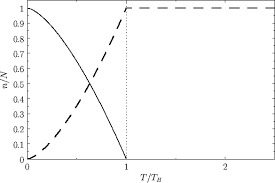
\includegraphics[width=0.7\textwidth]{fig6}
    \end{adjustbox}

    \begin{adjustbox}{center,caption={},label={somelabel},nofloat=figure,}
        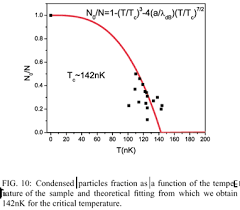
\includegraphics[width=0.7\textwidth]{fig7}
    \end{adjustbox}
      \ \ \ \ \ \ \ \ \ \ \ \ \ \ \ \ \ \ \ \ \  Bose Einstein Condensation graph
    \newpage
    \section*{Section - 5}
    \subsection*{Einstein's papers on the basis of Bose-Einstein statistics}
    \noindent
    --------------------------------------------------------------------------------------------------- \\ 
    \\
    \\
    \\
    \subsection*{The Quantum theory of mono-atomic ideal gas}

    The phase space of an elementary structure (here of a monoatomic molecule) is divided with reference to a three dimensional 
    volume into "cells" of extension $h^{3}$.\\ 
    Then the phase space volume will be 
    
    \begin{equation}
        \phi = V \frac{4}{3}\pi (2mE)^{3/2}
    \end{equation}
    
    Now at the thermodynamic equilibrium, ther entropy,S will be 
    \begin{equation}
        S = - K log \ \sum_{sr} (P^{s}_{r} \ log \ P^{s}_{r})
    \end{equation}

    Therefore we get number of molecules(n) and Energy(E) in the form,  
    \begin{equation}
        n = \sum _{s} \frac{1}{e^{\alpha ^ {s}}-1}
    \end{equation}
    \begin{equation}
        E = c \sum _{s} \frac{s^{2/3}}{e^{\alpha ^ {s}}-1}
    \end{equation}

    where 
    \begin{equation}
        c  = (2m)^{-1}h^{2}(\frac{4}{3}\pi V)^{-2/3}
    \end{equation}

    and 
    \begin{equation}
        \alpha^{s} = A + Bs^{2/3}
    \end{equation}

    Now free energy of the system 
    \begin{align}
        F &= E - TS \\
        \therefore F &= kT{log \ \sum_{s}(1-e^{-\alpha s}) -nA}
    \end{align}

    The pressure of the gas 
    \begin{align}
        P &= \frac{\partial F}{\partial V} \\
        \therefore P &= \frac{2E}{3V}
    \end{align}

    Hence we obtain, the remarkable result that the relation between the kinetic energy and the pressure is exactly the same as in the
    classical theory, where it is derived from the Virial theorem.
    \newpage
    \section*{Summary}

    Some time in June 1924, Einstein received a letter from a Bengali physicist,
    Satyendra Nath Bose, who asked him politely to translate—if he believed it
    was worth it—and forward for publication a paper on the hypothesis of light
    quanta, which he had attached. Einstein complied and translated and sent
    to Zeitschrift für Physik Bose’s subsequently famous paper. To the published
    paper, he added the following commentary:
    In my opinion Bose’s derivation of the Planck formula signifies an
    important advance. The method used also yields the quantum theory of the ideal gas, as I will work out in detail elsewhere.
    In Bose’s paper we find, for the first time, a derivation of the factor
    \begin{equation}
        \frac{8 \pi \upsilon ^{2}V d\upsilon }{c^{3}} 
    \end{equation}
    starting from the quantization of energy (c is the speed of light in vacuum,
    V the volume). This expression gives the number of cells corresponding to
    frequencies between $\upsilon$  and $\upsilon$ + d$\upsilon$ or, in wave-theoretical terms, 
    the number of modes with frequency in that same range. With the average energy of a
    resonator of frequency $\upsilon$ (or of a normal mode) it constitutes Planck’s blackbody
    radiation law for the energy density r:
    
    \begin{equation}
        r(\upsilon, T)d\upsilon  = \frac{8\pi \upsilon ^{2}}{c^{3}}\frac{h\upsilon d\upsilon}{e^{h\upsilon/kT}-1}
    \end{equation}
    
    (k is Boltzmann’s constant and T the temperature). While several different ways
    had been found to derive the average energy of a resonator based on Planck’s
    quantum hypothesis, the prefactor had previously been derived only classically,
    without invoking the concept of quantization. 

    Therefore, Bose’s manuscript was timely: After the experimental successes
    by Arthur Compton and Peter Debye, which seemed to confirm that light quanta
    have momentum as well as energy; after the spectacular discovery of Otto
    Stern and Walther Gerlach, for many physicists—Einstein among them—the
    most striking and convincing demonstration of quantization; and shortly after
    Einstein’s return to his own research on light quanta. Probably for this reason
    it took him so little time to prepare a presentation in which he applied Bose’s
    method to an ideal gas. He presented it at the Prussian Academy on 10 July,
    only a month after Bose had signed his letter.
    In this paper we find the density of states of (kinetic) energy E for a molecule
    of mass m of an ideal gas:
    \begin{equation}
        2\pi \frac{V}{h^{3}}2m^{3/2}E^{1/2}dE 
    \end{equation}
    

    It gives the number of phase cells of a single molecule corresponding to energies between E and 
    E + dE. Following Bose’s derivation, Einstein maximized the probability of a certain distribution
    of molecules in phase space, which he had previously divided into cells of volume $h^{3}$. He also took into account 
    only how many molecules were in each cell, not which, and introduced the constraint of the total number of particles, 
    a condition that is not invoked in the case of light quanta. He obtained the average occupation number of a state with 
    energy E, and also the equation of state of
    the ideal gas:

    \begin{equation}
        P = \frac{2E}{3V}
    \end{equation}

    \subsection*{The Second Paper}
    The second paper presents further detailed analysis of the consequences implied
    by the theory expounded in the first paper. Einstein emphasized this fact by
    numbering both equations and paragraphs in consecutive order with the first
    one.
    The most famous results of Einstein’s theory are contained in this
    paper. In this paper indeed, Einstein took the theory considerably further than
    Bose had done.

    First, Einstein discussed an unusual consequence: the condensation at low
    temperatures or, in other words, the saturated gas. Einstein considered, for the
    first time, the case of a gas in which, below a certain critical temperature (that
    depends on N and V ), the number of particles in excited states is limited. In the
    next section, he discussed the loss of statistical independence of the molecules
    in a famous passage where Ehrenfest’s name appears: \\ 
    "Mr. Ehrenfest and other colleagues have raised the criticism that in
    Bose’s theory of radiation and in my analogous theory of ideal gases
    the quanta or molecules are not treated as statistically independent
    entities without explicit mentioning of this feature in our respective
    papers. This is entirely correct." \\ 
    And the passage continues: \\
    "If the quanta are treated as statistically independent regarding their
    localization, one obtains Wien’s law of radiation; if one treats the gas
    molecules in an analogous way, one arrives at the classical equation
    of state, even if one proceeds in exactly the same way as Bose and I
    have done. " \\ 
    Then, Einstein elucidated this issue analytically, but he left in the dark
    what kind of dependence it is that affects the behaviour of molecules in the
    new statistics. He pointed out something that he had already suggested in his
    previous paper: In classical theory the entropy expression forces one to choose
    between two different conditions to be fulfilled, that is, Nernst’s principle or the
    extensivity of entropy. In the new theory, the two conditions are satisfied at the
    same time. Einstein considered this fact a strong support of the deep analogy
    between radiation and gas on which his theory was founded: \\ 

    "For these reasons I believe that one has to prefer the conception a)
    (i.e., Bose’s statistical approach) even if this preference over others
    cannot be justified apriori. This result in itself lends support for the
    belief in the deep essential similarity between radiation and gas in
    that the same statistical conception that leads to Planck’s formula
    produces the agreement between gas theory and Nernst’s theorem
    when applied to ideal gases." \\ 

    Also in this paper, we find the first appeal by Einstein to a certain duality
    in terms of the thesis by Louis de Broglie. After analyzing the energy fluctuations 
    of an ideal gas, he described the ideas of the French physicist aimed at
    overcoming the opposition between waves and particles. The great impact this
    reference by Einstein to de Broglie’s work had on the research of Schrödinger
    has been noted on many occasions, as Schrödinger never failed to recognize it.
    Appealing to the wave field that would accompany each particle, Einstein proposed to solve the paradox with which he had
    closed the previous paper: The
    interference will only take place in gases composed of molecules of equal mass. \\ 

    We regard Einstein’s second paper on the quanta a milestone in the history
    of quantum physics, not only because of the unusual amount of new results
    it contains but also because in a certain sense it closed the circle that was
    initiated by Einstein himself twenty years earlier with his heuristic hypothesis
    of light quanta. He was a pioneer in emphasizing the dual nature of radiation in
    1909. In 1925, with a completely analogous procedure, he in turn demonstrated
    the validity of his proposal for the ideal gas.
    In short, Einstein developed the analogy between gas and radiation, knowing
    that despite the evidence he could adduce to support the theory, it was unsure
    whether his theory was the true theory. In his own words: \\ 
    
    " The interest in this theory derives from the fact that it is based on
    the hypothesis of an extended formal similarity between radiation
    and gas. According to this theory, the degenerate gas differs from
    the gas of mechanical statistics in an analogous way as the radiation
    according to Planck’s law differs from the radiation according to
    Wien’s law. If one takes Bose’s derivation of Planck’s radiation
    formula seriously, then one cannot ignore this theory of the ideal gas
    either; because if it is justified to conceive of the radiation as a gas
    of quanta, then the analogy between a gas of quanta and a gas of
    molecules must be a complete one." \\ 

    In the third paper, Einstein insisted on this
    analogy in order to obtain new arguments for the validity of the theory. \\ 
    
    Einstein’s third paper is implicitly a response to Ehrenfest’s
    scepticism toward Einstein’s new theory. \\

    It is very likely that Einstein referred to these debates in Leiden in the comment in his 1925 paper in which he referred to Ehrenfest’s objections. This
    does not mean that the “others” Einstein mentioned were the Russian friends of
    Ehrenfest. At least, the Austrian physicist Otto Halpern had pointed out to Einstein the lack of statistical independence of the molecules in the new approach.
    He sent Einstein a detailed explanation of how the statistical independence of
    the elements under consideration had statistical implications. As he himself
    says, he based his reflections on Ehrenfest’s and Krutkow’s previous works. In
    his response, Einstein who admits Halpern had “illuminated very clearly a point
    of essential significance”distinguishes between two hypotheses: \\ 

        1) All distributions of the individual quanta over the “cells” are
        equally probable (Wien’s law). \\ 
        2) All different quantum-distribution-pictures over the “cells” are
        equally probable (Planck’s law). \\

    And he continued:\\
    
    Hypothesis 2 doesn’t square with the hypothesis of the independent
    distribution of individual quanta—but expresses, in the language of
    the theory of existing quanta—a mutual dependence of the latter
    among each other.
    Without experience one cannot decide between (1) and (2). The
    concept of independent atom-like quanta calls for (1), but experience demands (2). Bose’s derivation therefore cannot be regarded
    as a genuine theoretical justification of Planck’s law, but only as a
    reduction of that law to a simple, but arbitrary statistical elementary
    hypothesis. \\ 

    Referring to his own extension of Bose’s results to material gases, Einstein
    wrote: \\ 

    "This therefore also entails the implicit presupposition of certain statistical dependencies between the states of the molecules, a presupposition which the gas theory as such does not suggest. It would
    therefore be all the more interesting to know whether real gases behave according to this theory." \\ 
    
    \subsection*{The Third Paper}
    On 29 January 1925, Einstein presented the third and last paper of his quantum
    theory of the monatomic ideal gas to the Prussian Academy for publication
    in its Proceedings. This time, the sections and equations were not labelled
    consecutively with those of the preceding paper. Below we will return to this
    question in more detail, but these external aspects already suggest that the third
    contribution represents a path disconnected from the previous treatments. Or,
    at least, it seems Einstein wanted to present it this way. \\ 
    
    
    Einstein stated in the beginning that his theory was justified on the assumption that a light quantum differs, apart from polarization, from a material gas
    molecule only in the vanishing of its rest mass. This assumption was not taken
    for granted by many of his colleagues, nor had many researchers already accepted the statistical method used by Bose and by him.\\ 

    In this paper, Einstein did not assume that collisions between molecules be
    governed by the laws of mechanics. He asserted that if that would be the case,
    one would arrive at Maxwell’s distribution law and the classical equation of
    state. In fact, he neglected interactions among molecules, as is
    appropriate for an ideal gas; we must add that it is not true that all kinds of
    mechanical interactions lead to Maxwell’s distribution: we shall assume that
    Einstein was referring only to elastic collisions. \\

    What Einstein really wanted to emphasize is that, this interpretation implies
    that the entropy cannot be negative. If we consider the Sackur-Tetrode equation
    of state of an ideal gas,

    \begin{equation}
        S = N_{k}[log(\frac{2\pi mkT}{h^{2}})^{3/2}\frac{V}{N} + \frac{5}{2}]
    \end{equation}

    We see that, if the volume is small enough, the entropy would be negative. Does
    this mean that real gases, contrary to what is implied by Nernst’s theorem, can
    have negative entropies? No. It simply means that the classical theory of ideal
    gases can only be taken as valid under certain conditions. This is in analogy, so
    Einstein, to the case of Wien’s radiation law.

    \newpage
    \section*{Reference}
    (i) "Plank's law and light quantum hypothesis"  by S.N. Bose and Albert Einstein. \\ 
    published August, 1924.\\ 
    \\
    (ii) "Quantum Theory of monoatomic Ideal Gas" by A.Einstein \\
    published September, 1924\\
    \\
    (iii) "Quantum Theory of monoatomic Ideal Gas. Second Paper" by A.Einstein \\
    published February, 1925\\ 
    \\
    (iv) "On The Quantum Theory of the Ideal Gas" by A.Einstein \\
    published March, 1925\\ 
    \\
    (v) Classical and Statistical Thermodynamics \\
     - Ashley H. Carter.\\ 
     \\
    (vi) Statistical Mechanics \\
    - R. K. Pathria\\ 

    (vii) Planck’s radiation law, the light quantum, and the prehistory of indistinguishability 
    in the teaching of quantum mechanics.\\ 
     - Passon, Oliver; Grebe-Ellis, Johannes (2017) \\ 

    (viii) Superconductivity, Superfluids and Condensates. 
     - Annett, James F. (2004).\\

    (ix) Introduction to Quantum Mechanics (2nd ed.). \\
     - Griffiths, David J. (2005).\\

    (x) Statistical Mechanics (1st ed.)\\
     - McQuarrie, Donald A. (2000)\\
\end{document}
